\section{Closeness}
\FloatBarrier
\begin{figure}[h]
	\centering
	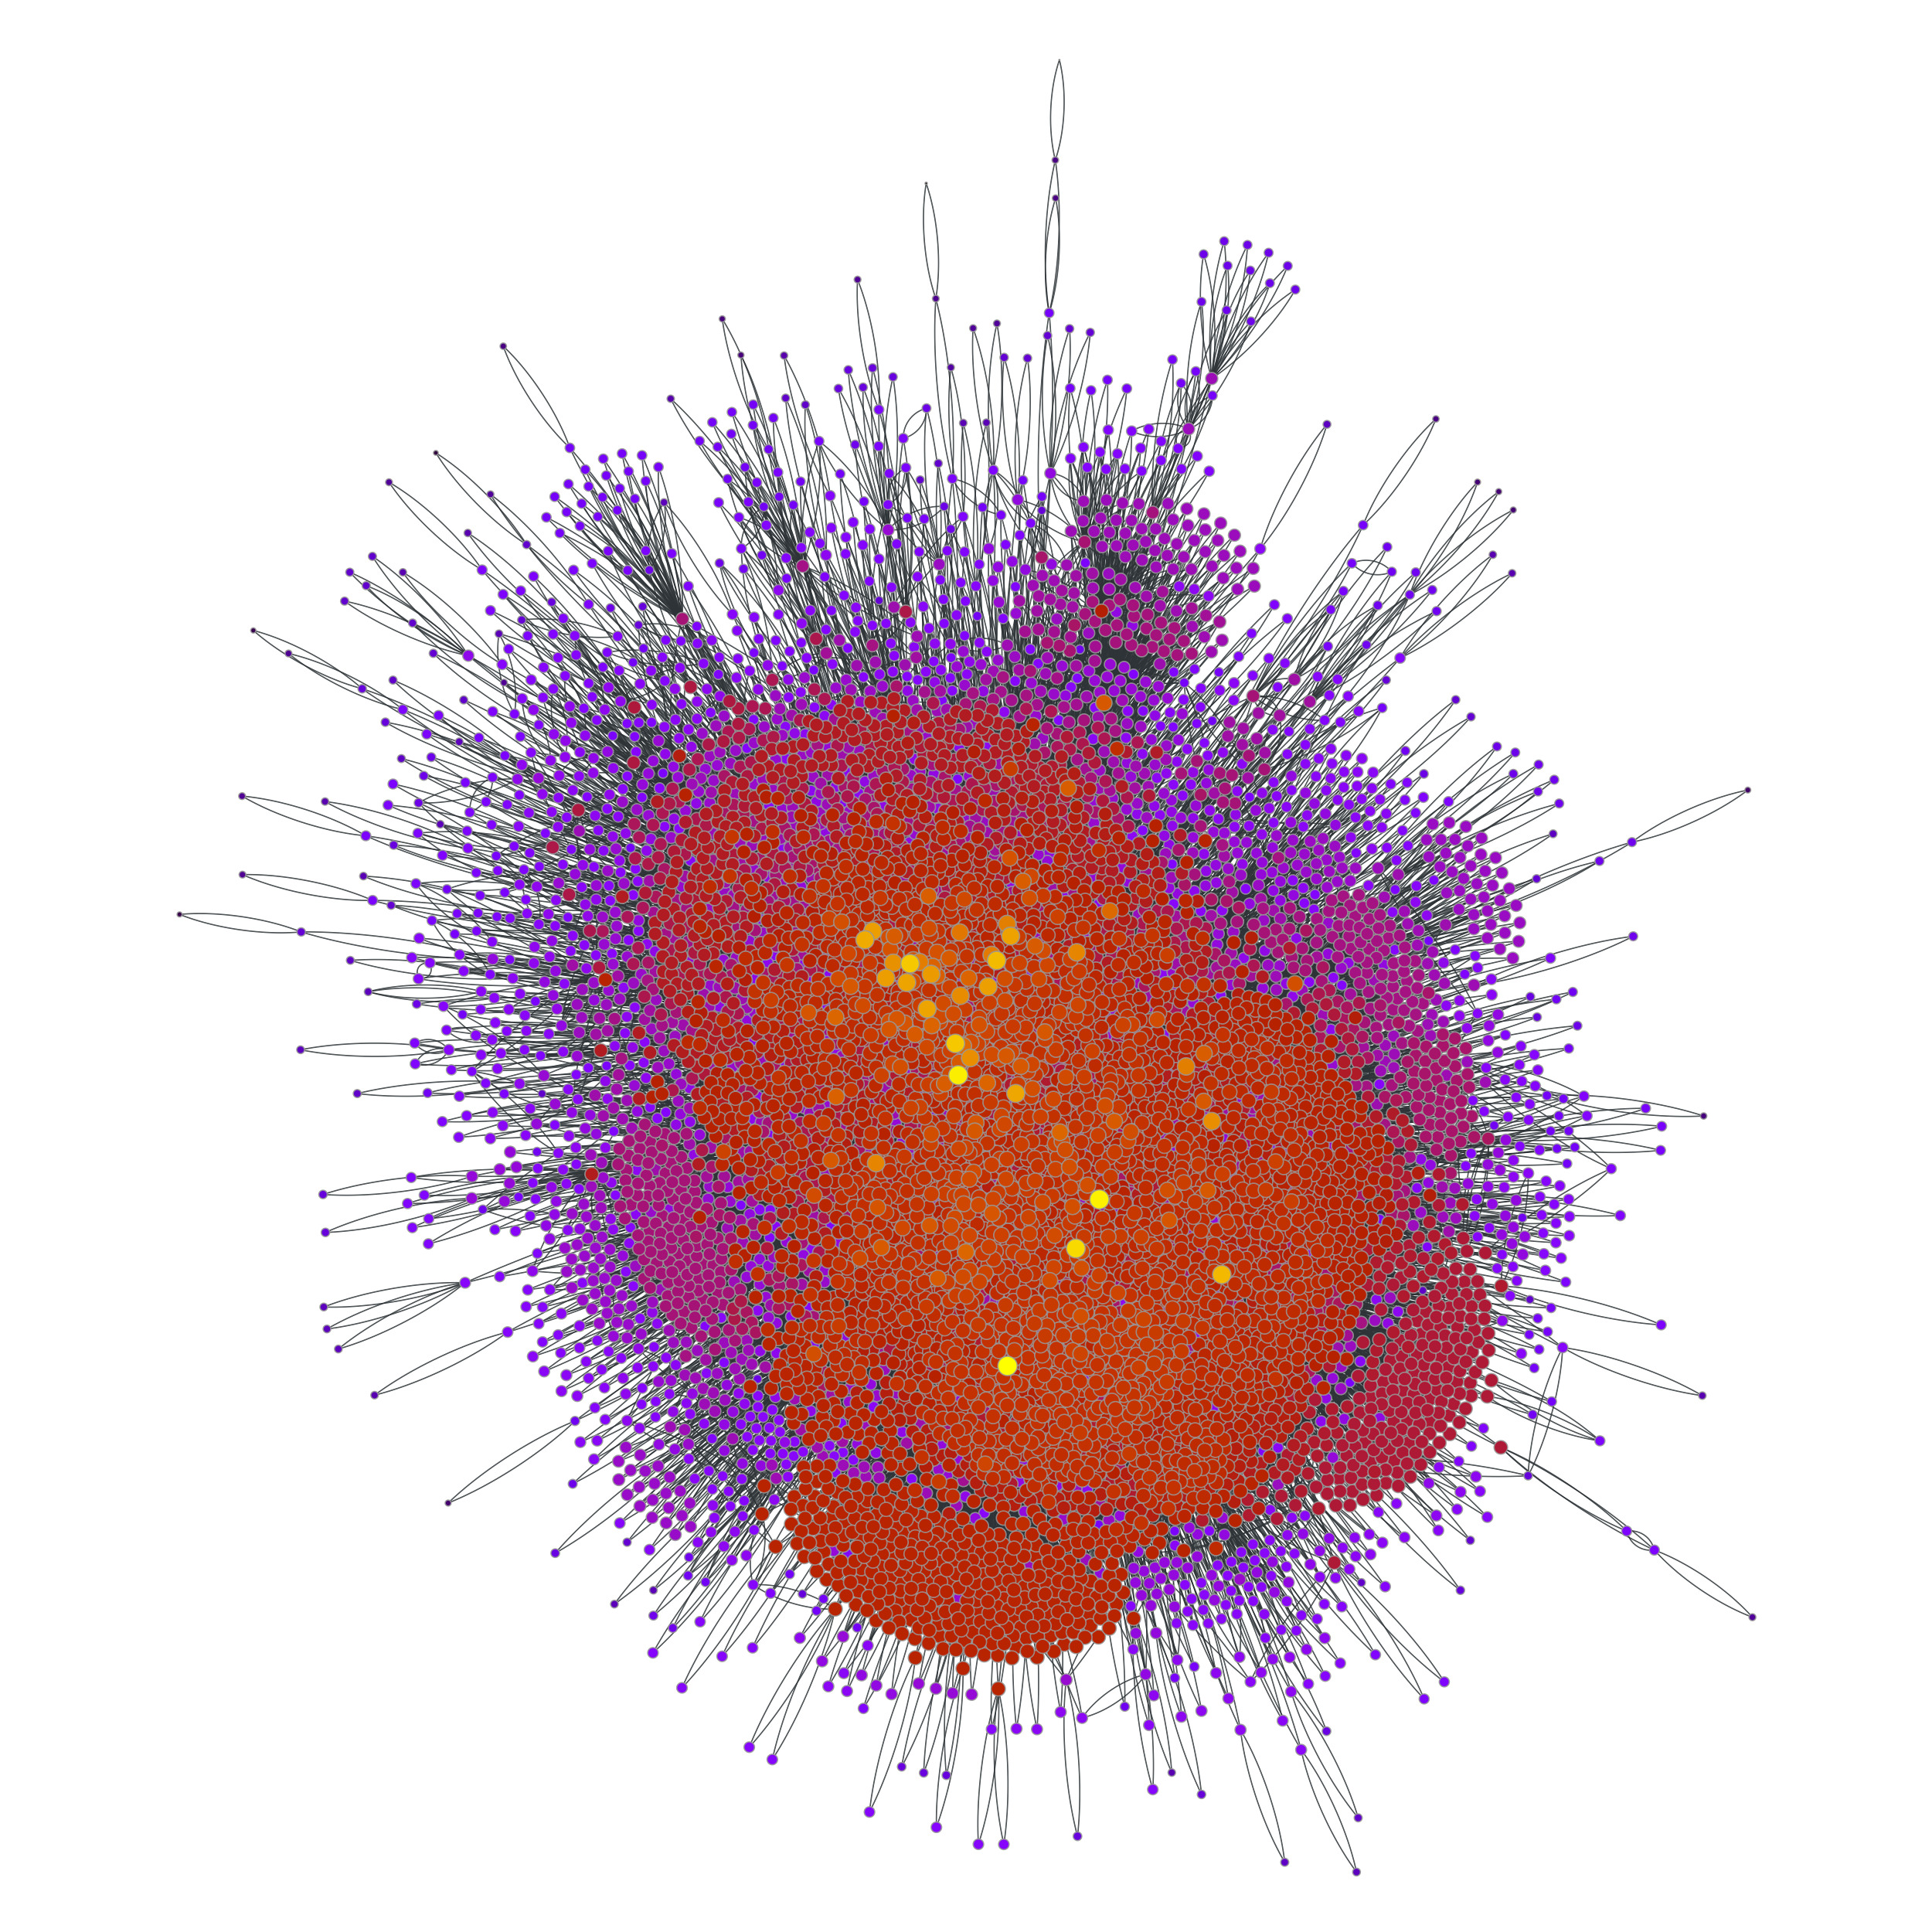
\includegraphics[width=\textwidth]{closeness_8k}
	\caption{Działanie algorytmu closeness na przykładowym grafie}
\end{figure}
\FloatBarrier
Powyżej przedstawione jest działanie algorytmu closeness na wybranym grafie. Kolor oraz wielkość wierzchołka zależy od wyniku algorytmu. Duże i jasne wierzchołki są wierzchołkami, z których najłatwiej dostać się do innych - wymagają średnio najmniej przeskoków by dostać się do innego wierzchołka. Przekłada się to bezpośrednio na to, że dany wierzchołek - fragment sieci może być często wybierany jako pośrednik.
\FloatBarrier
\begin{figure}[h]
	\centering
	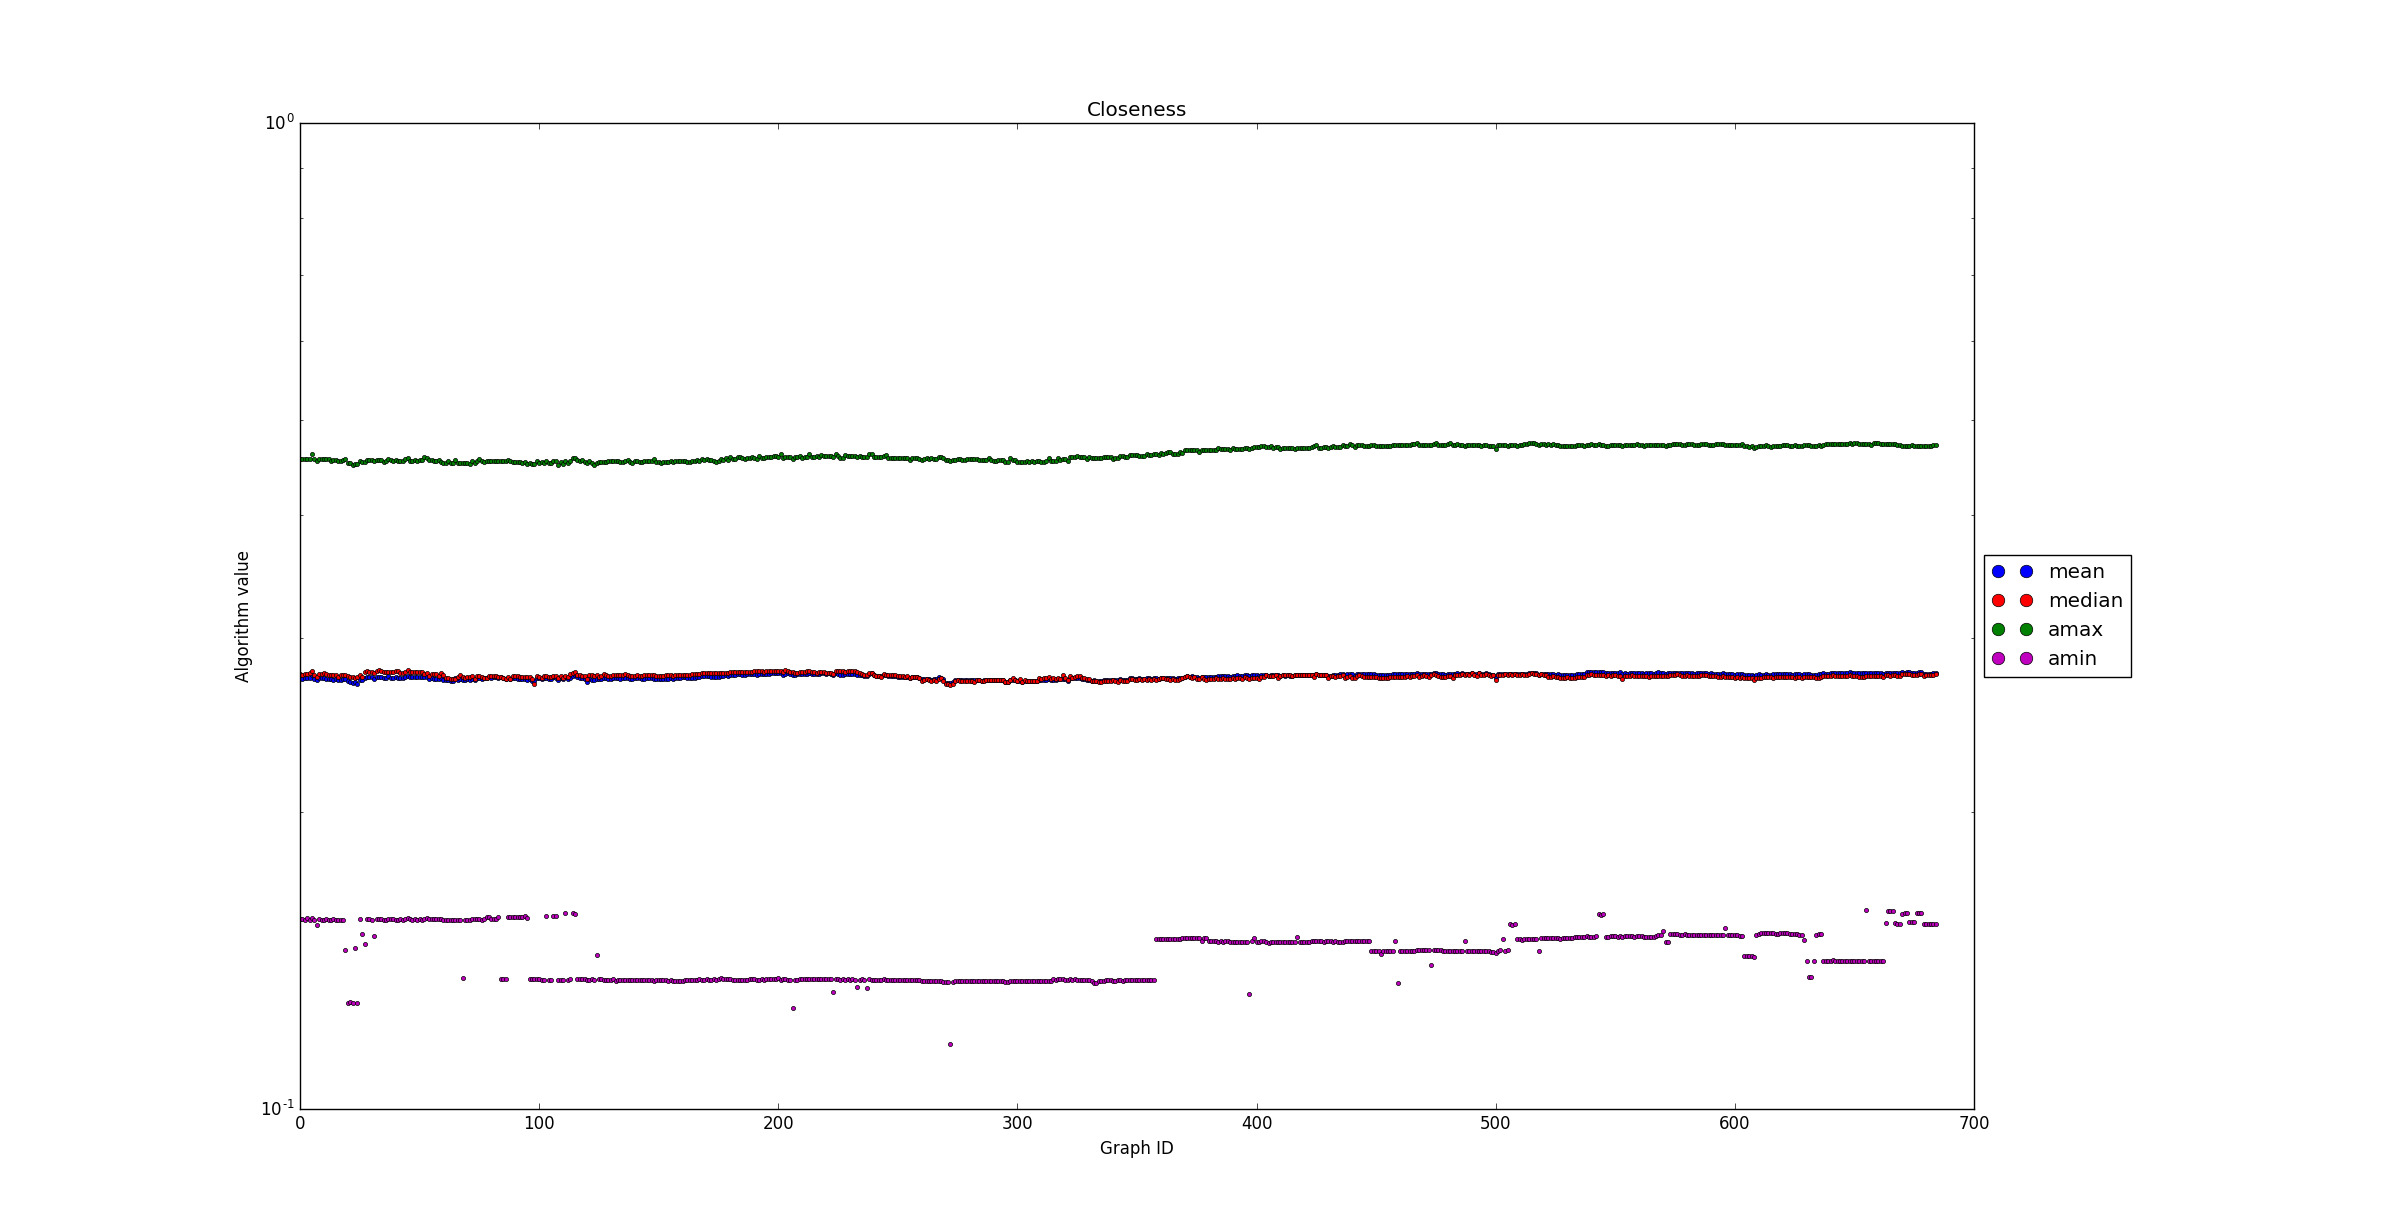
\includegraphics[width=\textwidth]{closeness}
	\caption{Wyniki algorytmu closeness}
\end{figure}
\FloatBarrier\FloatBarrier
\begin{figure}[h]
	\centering
	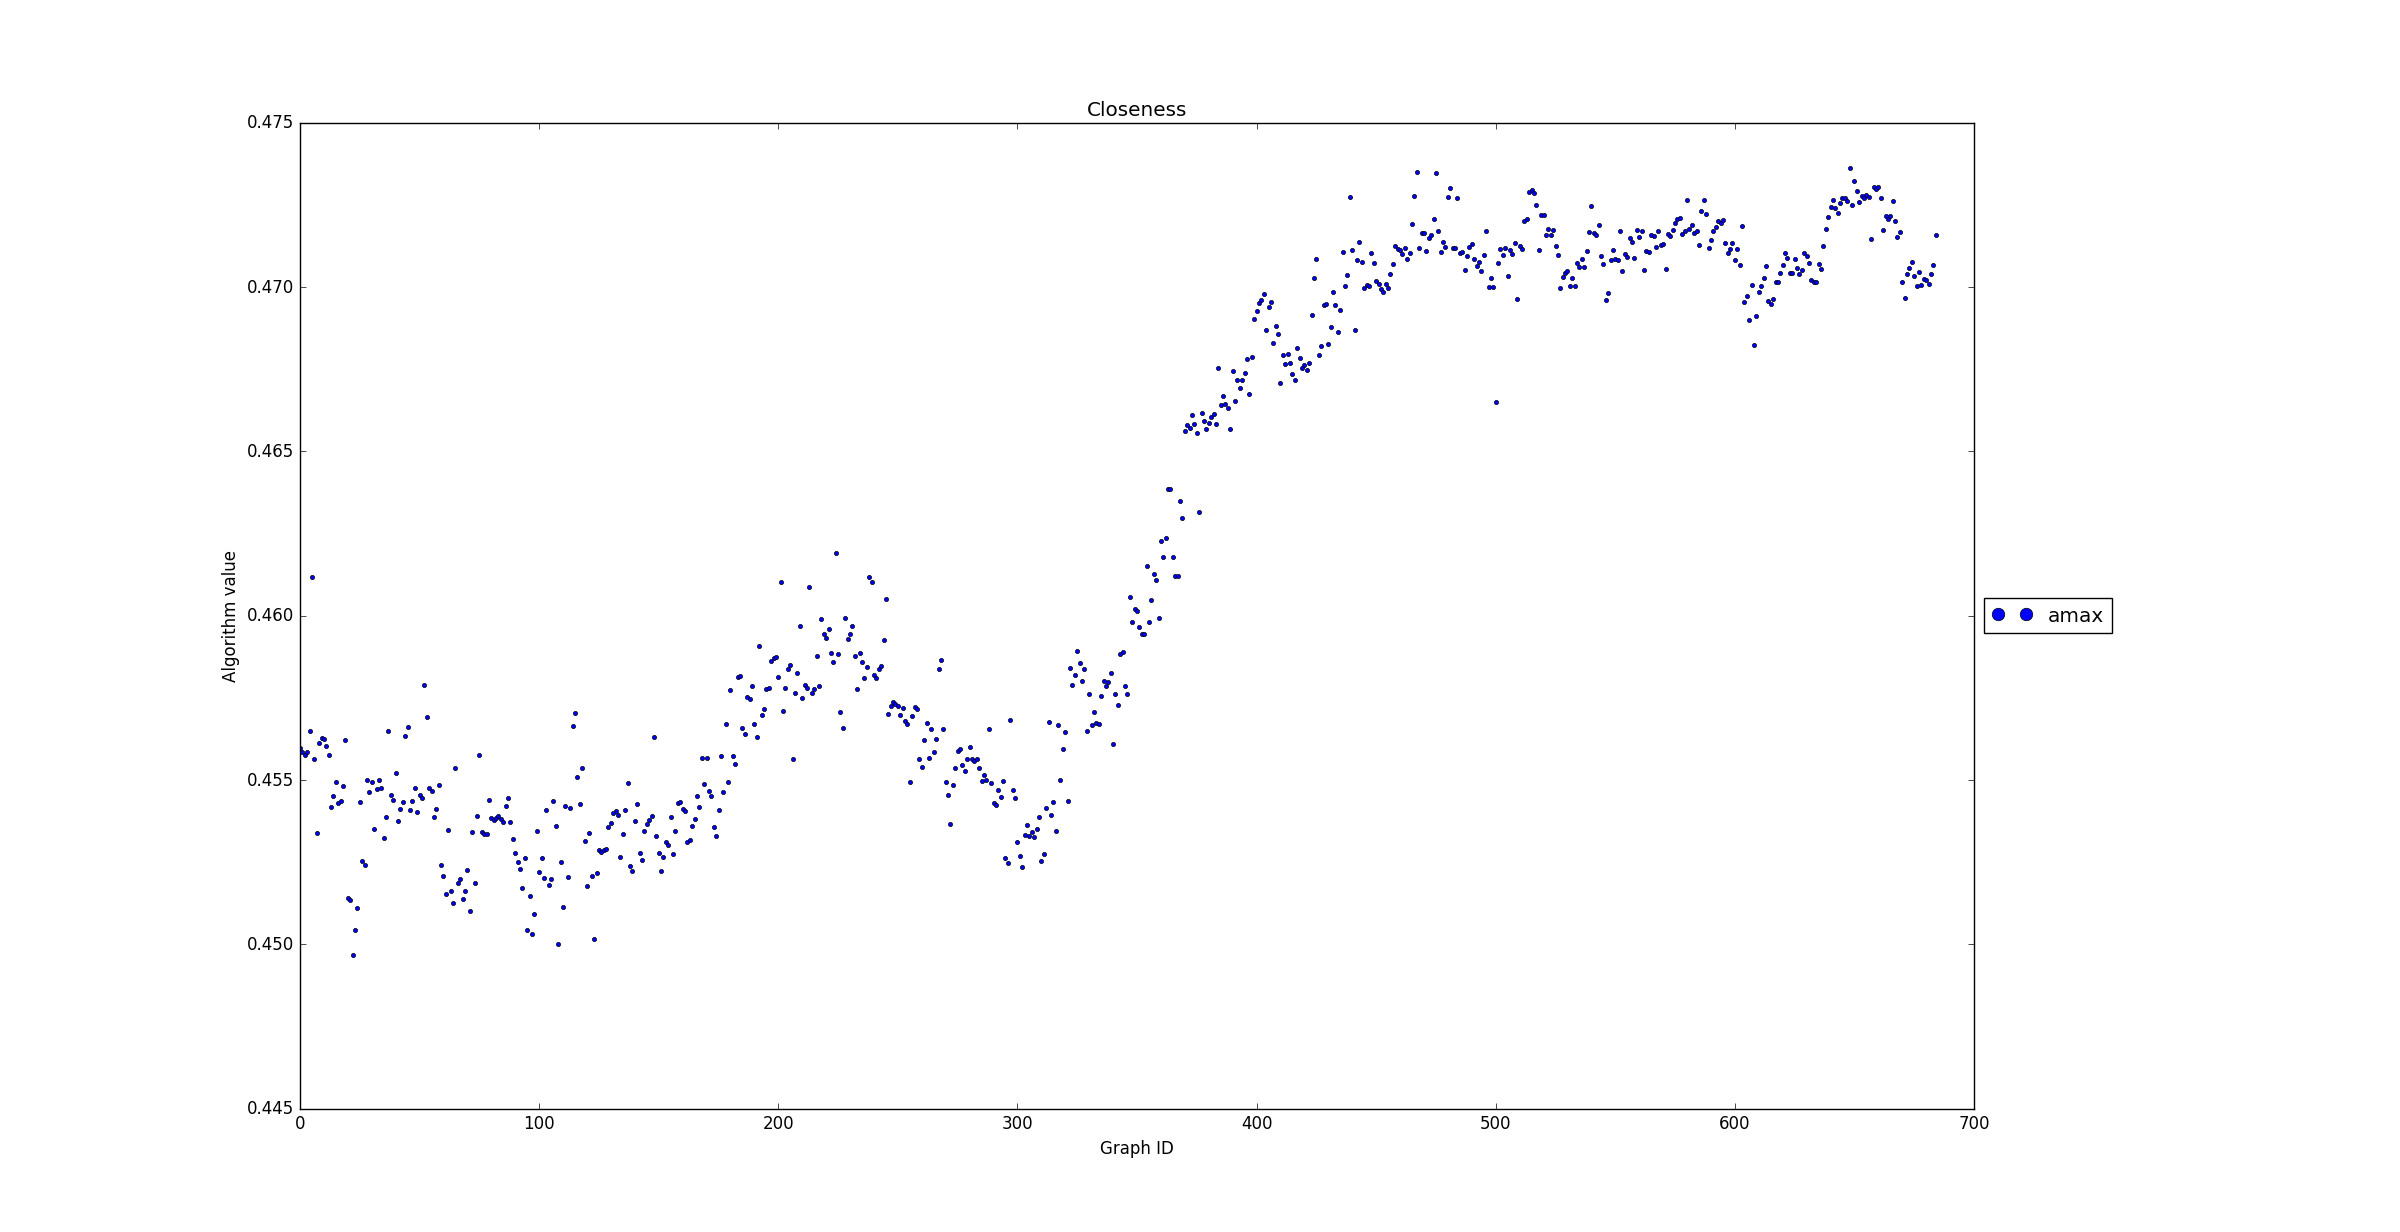
\includegraphics[width=\textwidth]{closeness_max}
	\caption{Maksymalne wartości closeness}
\end{figure}
\FloatBarrier\FloatBarrier
\begin{figure}[h]
	\centering
	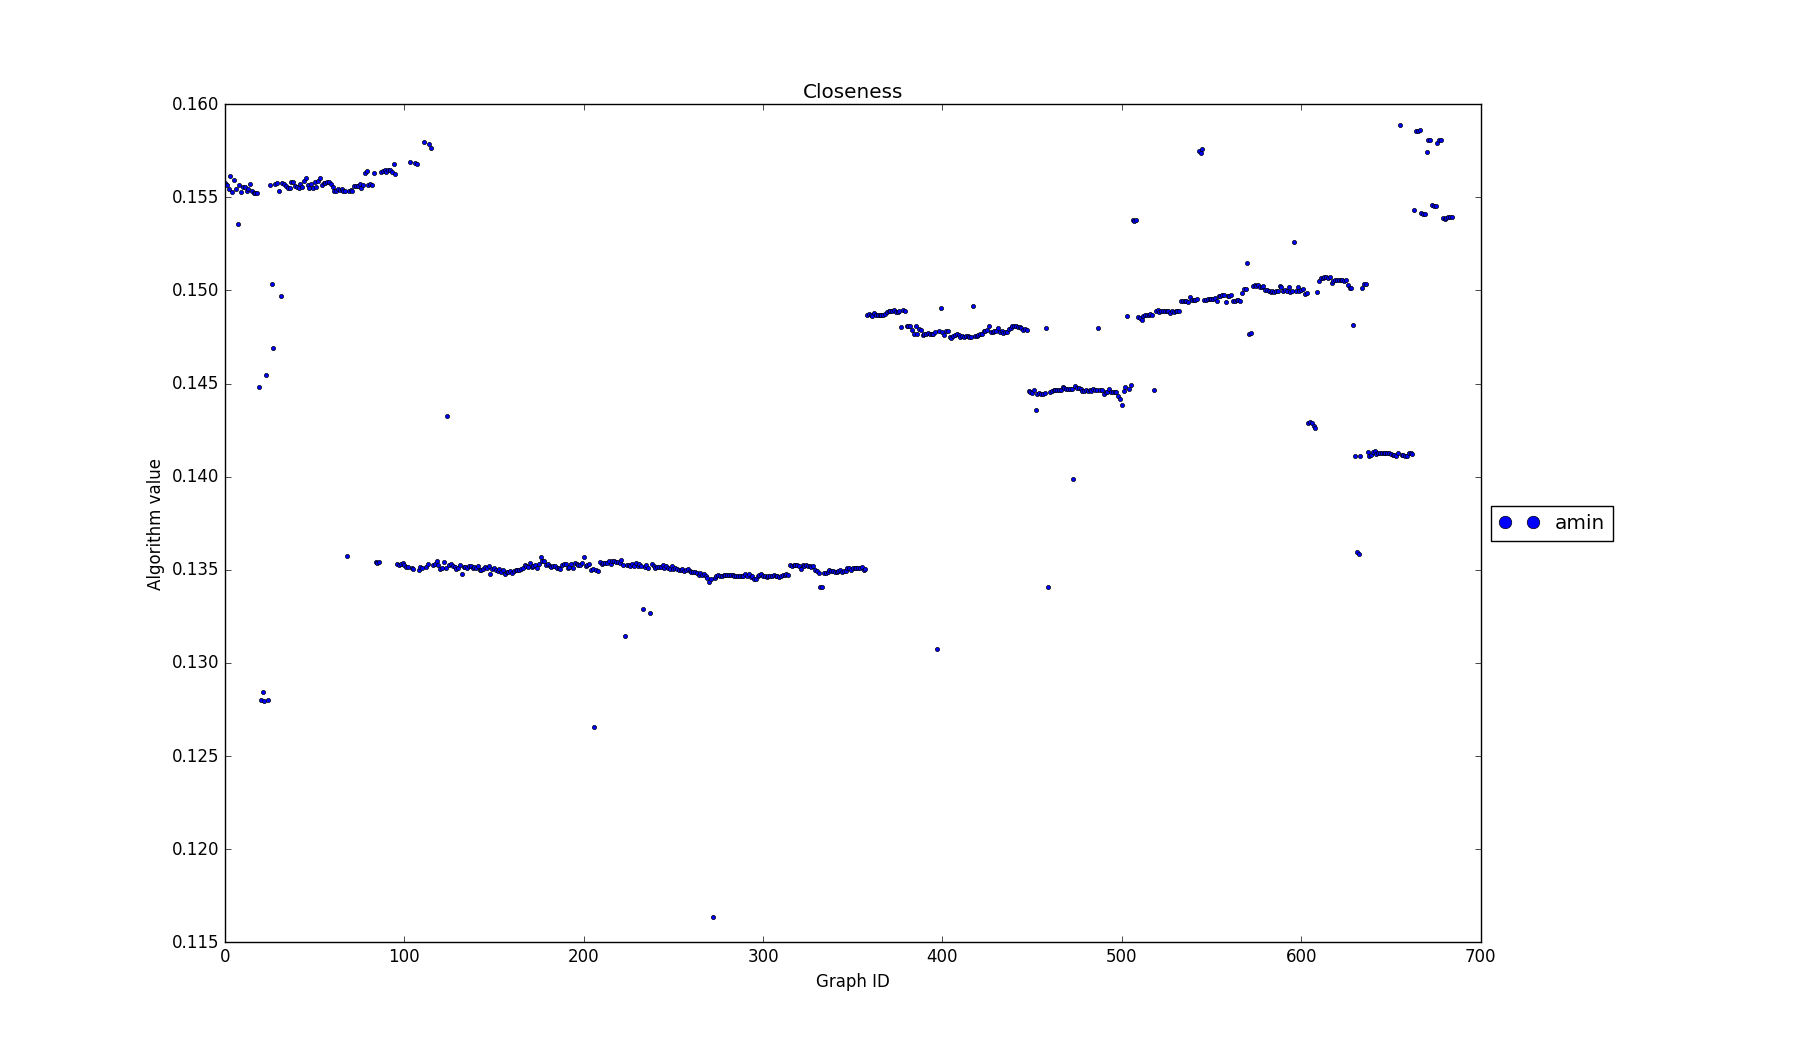
\includegraphics[width=\textwidth]{closeness_min}
	\caption{Minimalne wartości closeness}
\end{figure}
\FloatBarrier\FloatBarrier
\begin{figure}[h]
	\centering
	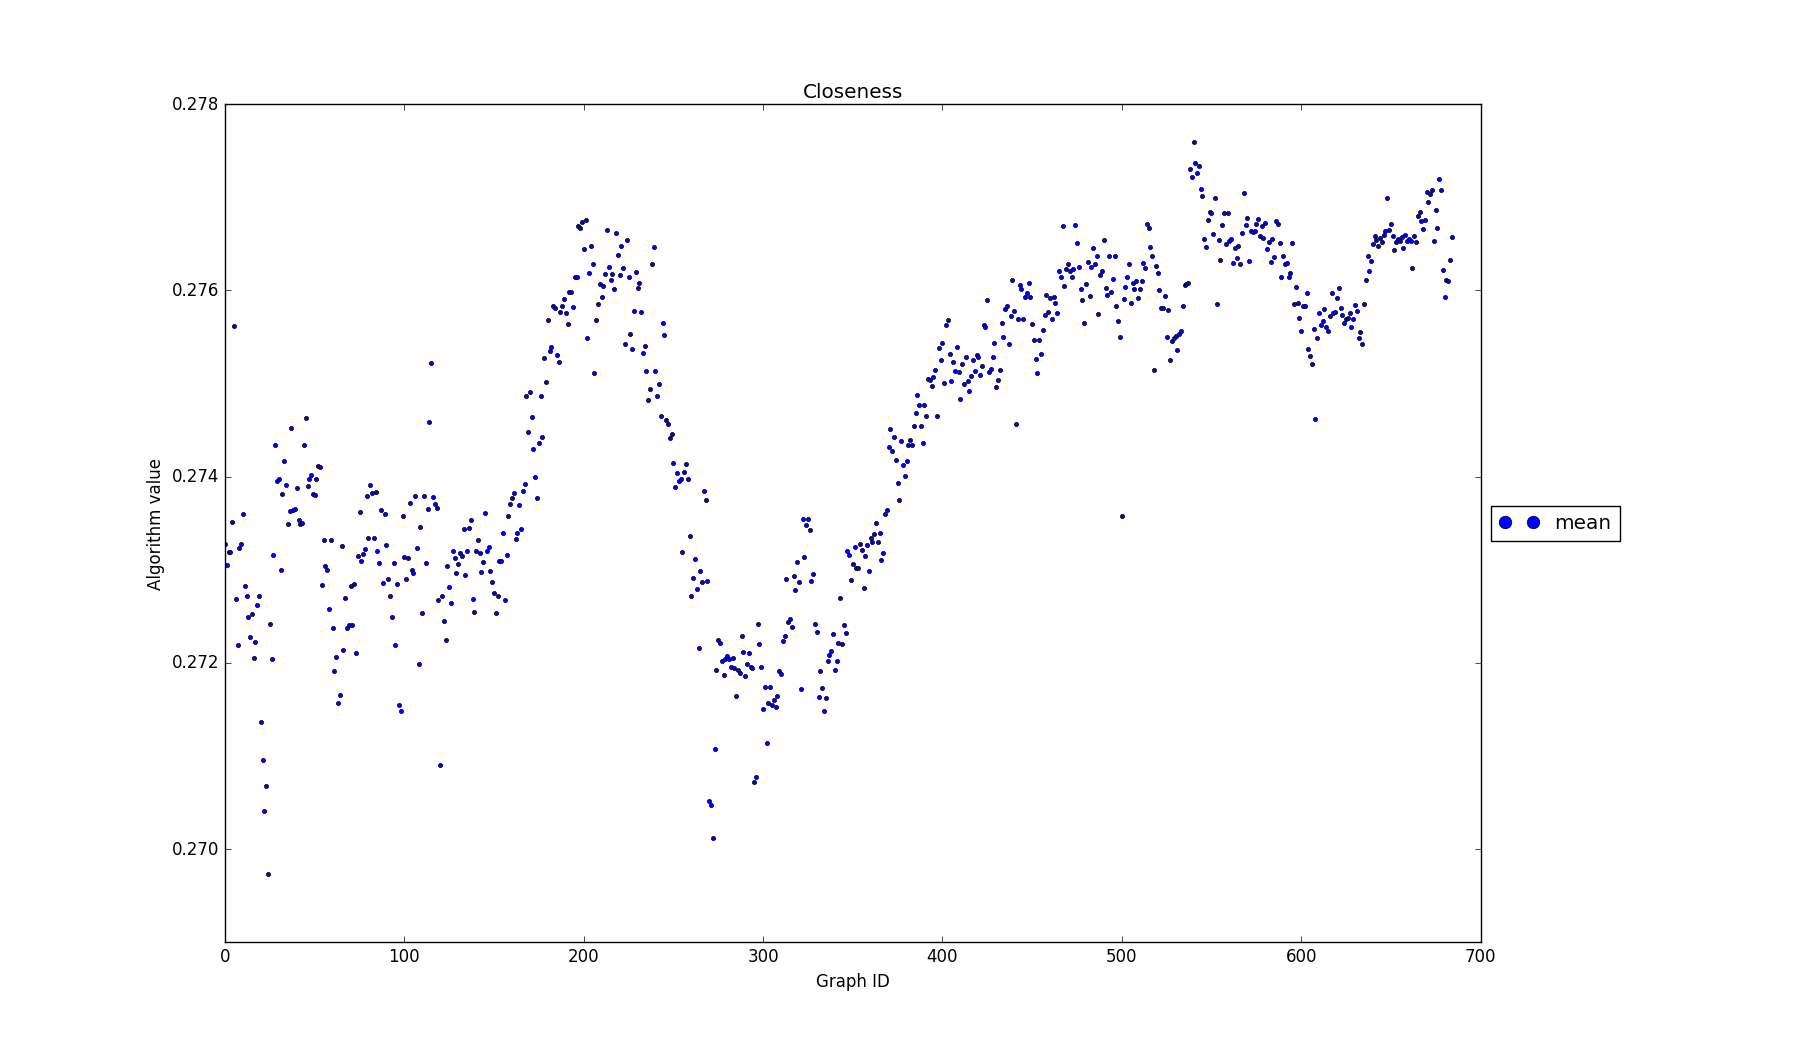
\includegraphics[width=\textwidth]{closeness_mean}
	\caption{Średnie wartości closeness}
\end{figure}
\FloatBarrier\FloatBarrier
\begin{figure}[h]
	\centering
	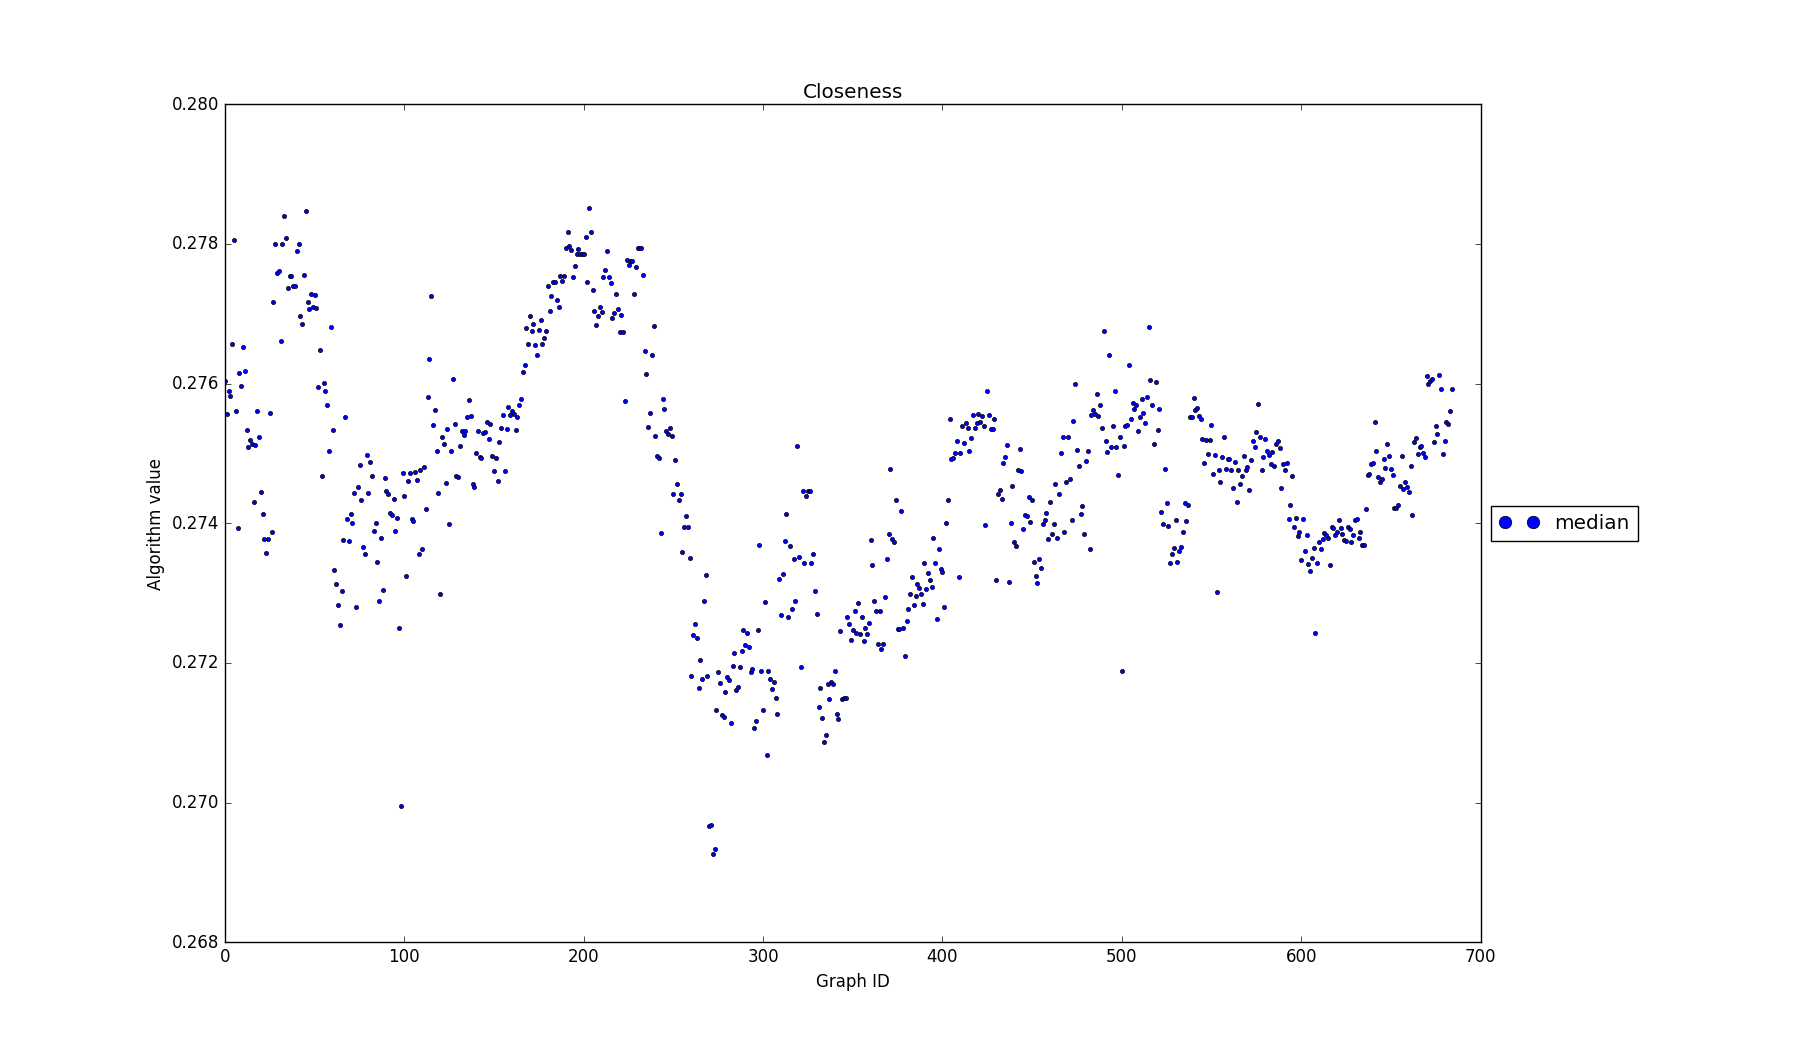
\includegraphics[width=\textwidth]{closeness_median}
	\caption{Mediana wartości closeness}
\end{figure}
\FloatBarrier
\newpage